\section{GPU 정보 확인하기}

\begin{enumerate}[label= (\alph*)]

    \begin{figure}[t]
        \centering
        \begin{subfigure}[b]{\textwidth}
            \centering
            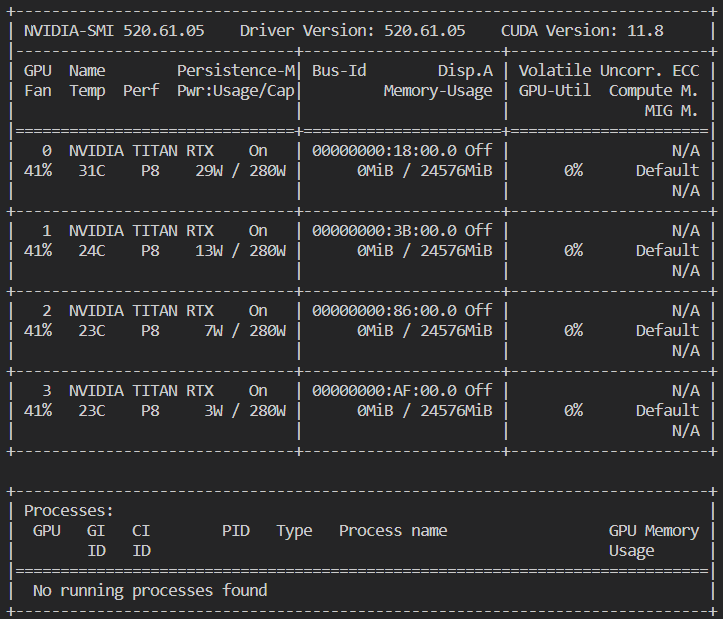
\includegraphics[width=0.55\textwidth]{imgs/srun_nvidia_smi.png}
            \caption{
                \texttt{srun --partition=class1 --gres=gpu:4 nvidia-smi} 커맨드 실행 결과.
            }\label{fig:srun_nvidia_smi}
        \end{subfigure}
        \hfill
        \begin{subfigure}[b]{\textwidth}
            \centering
            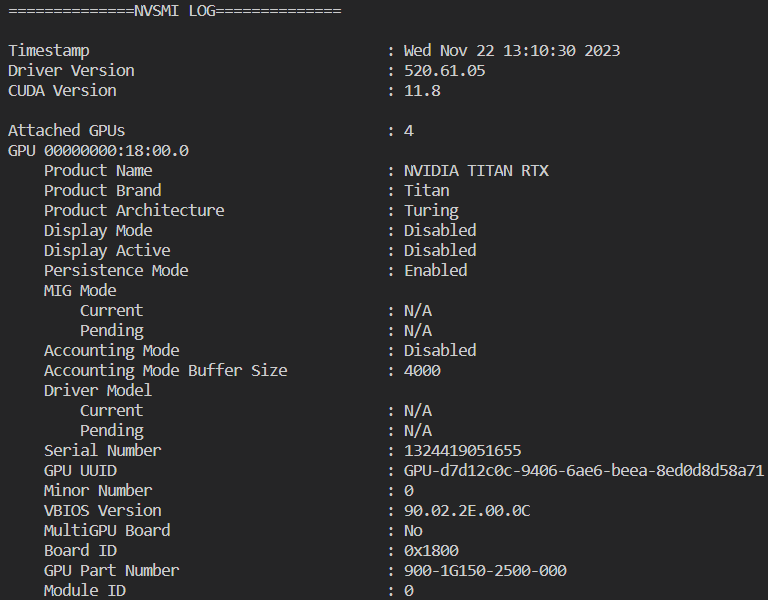
\includegraphics[width=0.55\textwidth]{imgs/srun_nvidia_smi_q.png}
            \caption{
                \texttt{srun --partition=class1 --gres=gpu:4 nvidia-smi -q} 커맨드 실행 결과.
            }\label{fig:srun_nividia_smi_q}
        \end{subfigure}
        \hfill
        \begin{subfigure}[b]{\textwidth}
            \centering
            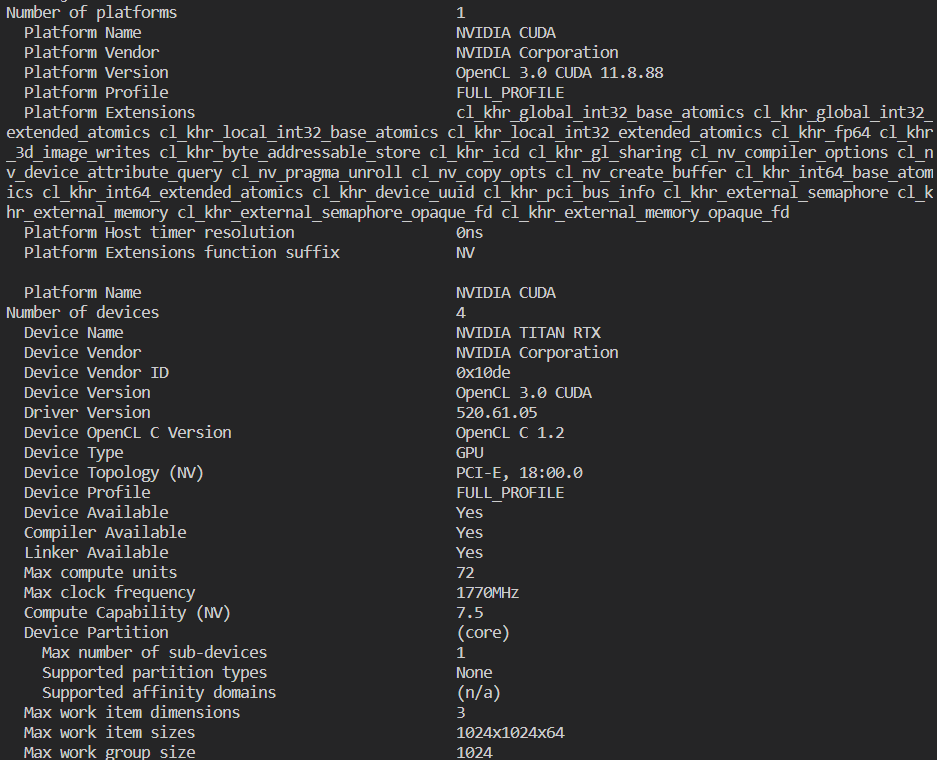
\includegraphics[width=0.55\textwidth]{imgs/srun_clinfo.png}
            \caption{
                \texttt{srun --partition=class1 --gres=gpu:4 clinfo} 커맨드 실행 결과.
            }\label{fig:srun_clinfo}
        \end{subfigure}
        \caption{각종 커맨드를 실행한 결과.}\label{fig:srun}
    \end{figure}

    \item {
        주어진 명령을 수행하여 Fig.~\ref{fig:srun}과 같은 출력을 얻었다. 긴 출력의 경우 앞부분만 첨부하였다.

        첫 번째 명령어는 4개의 GPU를 할당받아 \texttt{nvidia-smi}를 실행한 결과이다.
        \texttt{nvidia-smi}는 NVIDIA System Management Interface로, NVIDIA GPU를 관리 및 모니터링하는 도구이다.
        Fig.~\ref{fig:srun_nvidia_smi}에서 볼 수 있듯이, 4개의 GPU가 할당되었고 각 GPU의 상태를 확인할 수 있다.

        두 번째 명령어는 4개의 GPU를 할당받아 \texttt{nvidia-smi -q}를 실행한 결과이다.
        \texttt{-q} 옵션은 query 명령어로, 각 GPU의 상태를 더 자세히 확인할 수 있다.
        Fig.~\ref{fig:srun_nividia_smi_q}에서 볼 수 있듯이, 4개의 GPU가 할당되었고
        각 GPU의 세부 정보를 제공하고 있다. 굉장히 긴 출력이므로, 여기서는 앞 부분만 첨부하였다.

        세 번째 명령어는 4개의 GPU를 할당받아 \texttt{clinfo}를 실행한 결과이다.
        \texttt{clinfo}는 OpenCL을 지원하는 플랫폼 및 디바이스의 정보를 출력하는 도구이다.
        Fig.~\ref{fig:srun_clinfo}에서 볼 수 있듯이, CUDA 플랫폼을 인식하고 있으며
        4개의 GPU가 할당되었음과 각 GPU의 세부 정보를 확인할 수 있다.
        마찬가지로 굉장히 긴 출력이므로, 여기서는 앞 부분만 첨부하였다.
    }

    \item {
        이전 명령어의 출력들로부터 계산 노드에 장착된 GPU의 모델이 NVIDIA TITAN RTX임을 확인할 수 있다.
        노드당 장착된 GPU의 수는 4개이다.
    }

    \item {
        \texttt{nvidia-smi}의 출력을 통해 GPU의 global memory가 24576 MiB임을 확인할 수 있다.
        또한 \texttt{clinfo}의 출력을 통해 더 자세한 global memory의 크기를 알 수 있는데,
        25396969472 bytes임을 확인할 수 있다. 이는 앞서 확인한 24576 MiB에 근사한 수치이다.
    }

    \item {
        GPU의 maximum power limit은 \texttt{nvidia-smi}의 출력을 통해 280 W임을 확인할 수 있다.
        또한 maximum SM clock speed는 \texttt{nvidia-smi -q}의 출력을 통해 2100 MHz임을 확인할 수 있다.
    }

    \item {
        \texttt{clinfo}의 출력을 통해 Max work item dimension, Max work item size, Max work group size가
        각각 3, $(1024\times1024\times64)$, 1024임을 확인할 수 있다.
    }

\end{enumerate}